\documentclass[11pt]{article}
\usepackage[a4paper,margin=25mm]{geometry}
\usepackage{amsmath,amssymb,bm}
\usepackage{graphicx}
\usepackage{booktabs}
\usepackage{microtype}
\usepackage{xcolor}
\usepackage[colorlinks=true,allcolors=blue]{hyperref}
\hypersetup{pdftitle={Species volume fractions in granular mixtures from rotating radiography},pdfauthor={Benjy Marks}}
\graphicspath{{../figures/}}
\newcommand{\todo}[1]{\textcolor{red}{[#1]}}
\newcommand{\plan}[1]{\textcolor{blue!60!black}{\textit{Plan:} #1}}
\newcommand{\dd}{\mathrm{d}}
\newcommand{\x}{\bm{x}}
\newcommand{\q}{\bm{q}}

\title{Species volume fractions in granular mixtures from rotating radiography}
\author{Benjy Marks\\ \small The University of Sydney, Sydney, Australia\\ \small \todo{co-authors}}
\date{\today}

\begin{document}
\maketitle

\begin{abstract}
The solid fraction and the volume fraction of each grain size in a granular
mixture change during flow, through dilation and segregation, but X-ray
tomography resolves them only when the flow is stopped, and radiography
averages them along the beam. We show that the power spectrum of a small
patch of a radiograph of a dense packing is, in expectation, a line integral
of a local spectral density that is linear in the species volume fractions,
once grain interference is included through the partial structure factors
of the mixture. Radiographs taken from many directions by a rotating
cone-beam scanner therefore determine three-dimensional, time-dependent
fields of species volume fraction through a linear inverse problem, without
resolving grains or a reference scan. We test the method on synthetic
radiographs of evolving bidisperse sphere packings with exact cone-beam
projections. With about 600 large grains per element of the reconstruction
mesh, the solid fraction is recovered to 0.005 and the large-grain fraction
of the solid to 0.023 (root mean square over the specimen and the
sequence). The error of the large-grain field equals, without a fitted
parameter, the counting fluctuation of the grains in an element, which
gives the element size needed for a given accuracy. The errors are
insensitive to detector noise up to several per cent of the path length and
to the number of radiographs per turn, follow changes within a quarter turn,
and are up to four times smaller than those of fields constrained to vary
with height only. \todo{experimental validation}
\end{abstract}

% ---------------------------------------------------------------------------
\section{Introduction}

Segregation, dilation and compaction in flowing granular mixtures are
three-dimensional and change on the time scale of the flow. Their
measurement inside an opaque material has relied on X-ray tomography, which
needs the specimen to be still for the duration of a scan, so that flows are
stopped and restarted between scans \todo{cite: tomography of segregation or
dilation in stopped flows}. Radiography is fast but integrates through the
depth of the specimen: a layer of large grains in front of a layer of small
grains gives the same mean attenuation as a uniform mixture.

Two families of methods extract more than the mean from radiographs. Image
correlation methods follow the texture of the grains. Projection-based
digital volume correlation fits a space-time displacement field directly to
a sequence of radiographs taken while a scanner rotates, against a reference
volume from a full scan \todo{cite: projection-based DVC, Roux, Hild and
co-workers}. It requires the texture to persist, which it does not once
grains rearrange, and it measures displacement, not composition. Spectral
methods instead treat a radiograph of a dense packing as a random field. The
power spectrum of the projected path length through solid depends on the
grain size distribution, the solid fraction and the arrangement of the
grains, and its high-wavenumber part gives the solid fraction, the specific
surface and the volume fraction of each species without calibration
\todo{cite: spectral analysis of radiographs of granular media; pynamix}.
These estimates are averages along the beam.

Here we combine the second idea with the geometry of the first. A scanner
that rotates around a specimen, such as a gantry scanner, records each
point of the specimen from many directions while the material evolves. We
show that the spectrum of a detector patch is the sum of contributions from
every depth its rays cross, each linear in the local species volume
fractions, and use this to reconstruct the fields in three dimensions and in
time by linear least squares. Section~\ref{sec:method} gives the forward
model, the error model and the reconstruction.
Section~\ref{sec:synthetic} describes synthetic tests with exact projections
of evolving packings, and Section~\ref{sec:results} reports how the accuracy
depends on the number of grains per element, the detector, the size ratio
and polydispersity, the time resolution and the container wall.
Section~\ref{sec:experiments} is reserved for experiments.

% ---------------------------------------------------------------------------
\section{Method}\label{sec:method}

\subsection{Spectral density of a projected packing}

Let $I(\x)$ be the indicator of solid in a packing of spheres of species
$a$, with diameters $d_a$, volumes $v_a=\pi d_a^3/6$, number densities
$\rho_a$ and volume fractions $\phi_a=\rho_a v_a$. After flat-field
correction and linearisation, a radiograph gives the path length through
solid along each ray, $X(\bm\xi)=\int I\,\dd s$, at detector position
$\bm\xi$.

The three-dimensional spectral density of $I$, per unit volume and away
from zero wavenumber, is
\begin{equation}
\chi(k)=\sum_{a,b}\sqrt{\rho_a\rho_b}\,v_a v_b\,F(k d_a/2)\,F(k d_b/2)\,S_{ab}(k),
\label{eq:chi}
\end{equation}
where $F(u)=3(\sin u-u\cos u)/u^3$ is the amplitude form factor of a sphere
and $S_{ab}$ are the Ashcroft--Langreth partial structure factors of the
mixture \todo{cite: partial structure factors of mixtures}. With
$S_{ab}=\delta_{ab}$, Eq.~\eqref{eq:chi} reduces to the self term
$\sum_a\phi_a v_a F^2(k d_a/2)$, which describes grains placed independently.

In a cone beam a feature at a point $\x$ appears on the detector magnified
by $M(\x)$, the ratio of the source--detector distance to the distance from
the source to $\x$ along the detector normal. Consider a slab of the
specimen normal to the beam, of thickness $\dd s$ larger than the range of
the interference terms but small compared with the specimen. Its projection
has a two-dimensional spectral density equal to $\dd s$ times $\chi$
evaluated at the in-plane wavevector, by the projection-slice theorem.
Mapped to the detector, where an object wavenumber $k$ appears at $q=k/M$
and the area scales by $M^2$, a slab contributes $M^2\chi(qM)\,\dd s$.
Slabs separated by more than the interference range are uncorrelated, so
the expected spectral density of $X$ near a detector point is the integral
along its ray,
\begin{equation}
\mathbb{E}\,P(q)=\int M(\x)^2\,\chi\bigl(qM(\x);\x\bigr)\,\dd s,
\label{eq:additive}
\end{equation}
in which $\chi$ depends on position through the local composition. The
expected mean path length is $\mathbb{E}\,X=\int\phi\,\dd s$, with
$\phi=\sum_a\phi_a$.

Equation~\eqref{eq:chi} is quadratic in the number densities. We write it as
$\chi=\sum_a\phi_a\chi_a$ with
\begin{equation}
\chi_a(k)=F(kd_a/2)\sum_b\sqrt{\rho_b/\rho_a}\,v_b\,F(kd_b/2)\,S_{ab}(k),
\label{eq:chia}
\end{equation}
and evaluate $\chi_a$ at the mean composition of the specimen, using
Percus--Yevick partial structure factors \todo{cite: Percus--Yevick
closure for hard-sphere mixtures}. The spectral density is then linear in
the fields $\phi_a(\x)$. Section~\ref{sec:local} tests the effect of
evaluating $\chi_a$ at the local composition instead.

\subsection{Patch spectra}

Each radiograph is cut into square patches of $m$ pixels of pitch $p$. For
a patch we compute the windowed periodogram
$\hat P(\q)=p^2|\mathcal{F}[W(X-\bar X_W)]|^2/\sum W^2$, with $W$ a Hann window
and $\bar X_W$ the window-weighted mean, divide out the transfer function of
the pixel aperture, and average over annuli of width $2\pi/(mp)$. The
normalisation gives the spectral density in absolute units
\todo{cite: pynamix.spectral normalisation}. White detector noise of
variance $\sigma_n^2$ in $X$ adds $p^2\sigma_n^2$, which is subtracted.

The expectation of an annulus value is not $\mathbb{E}P$ at its mean
wavenumber. It averages $\mathbb{E}P$ over the annulus and over the
spectrum of the window, which spreads power across a few wavenumber bins.
Near the zeros of $F$ this averaging fills in the zeros, and leaving it out
overestimates the misfit by up to a third at the annuli used here. We therefore write the
expected value of annulus $b$ as $\sum_r\omega_{br}\,\mathbb{E}P(q_r)$ on a
fine grid of $q_r$, with weights $\omega_{br}$ computed once from the
window.

Within a patch, Eq.~\eqref{eq:additive} is averaged over a grid of rays.
The data for each radiograph are the patch means of $X$, from small patches,
and the annulus values in a band of wavenumbers, from larger patches.
Small patches resolve the solid fraction better, while the spectra need
patches that hold many grains.

\subsection{Space-time fields and the linear problem}

The fields are written on a regular mesh of trilinear hexahedral elements
times piecewise-linear functions of time,
\begin{equation}
\phi_a(\x,\tau)=w_a(\x)\sum_k\sum_n\psi_k(\tau)\,N_n(\x)\,c_{akn},
\label{eq:fields}
\end{equation}
where $\tau$ is the time of a radiograph within the sequence. The factor
$w_a$ describes the specimen surface. Grains whose centres fill a cylinder
straddle its surface, and the expected volume fraction of species $a$ falls
from its bulk value to zero over one grain radius on either side; for a
planar face at signed distance $s$ inside, $w_a=\tfrac12+\tfrac34 t-\tfrac14 t^3$
with $t=s/(d_a/2)$ clipped to $[-1,1]$, the fraction of a sphere of
diameter $d_a$ centred at the point that lies inside. The product over the
side and the two ends is used for a cylinder.

Substituting Eq.~\eqref{eq:fields} into Eq.~\eqref{eq:additive} and into the
mean gives the data as $G\bm c$, with $G$ assembled by sampling each patch's
rays. The kernel depends on position only through the magnification, so it
is tabulated in $M$ for each annulus and interpolated. The coefficients
minimise
\begin{equation}
(\bm d-G\bm c)^\top\Sigma^{-1}(\bm d-G\bm c)+\lambda\,\bar h\,\bm c^\top L\bm c,
\label{eq:ls}
\end{equation}
where $L$ is a discrete gradient penalty on the nodal values of each field,
$\bar h$ is the mean diagonal of $G^\top\Sigma^{-1}G$ and $\lambda=10^{-3}$.
The solid fraction, the large-grain fraction of the solid
$c=\phi_{\rm large}/\phi$ and the Sauter mean diameter
$d_{32}=\phi/\sum_a\phi_a/d_a$ follow from the fields.

The kernels of Eq.~\eqref{eq:chia} need the mean composition. The problem
is solved first with the self term, the mean volume fractions are taken from
that solution, and it is solved again with the interference terms.

\subsection{Error model}

The weights $\Sigma$ have two sources. An annulus value is the mean of $n_b$
periodogram bins, each exponentially distributed about its expectation, so
its variance is $(\mathbb{E}P+N_b)^2/n_b$, with $N_b$ the subtracted noise
spectrum. In addition, the number of grains under a patch fluctuates. A
patch mean then has a variance proportional to the number of grains along
its rays, and hence to $\bar X$; an annulus value has a relative variance
proportional to $1/\bar X$. The two grain-count terms have unknown scales.
They are set by iterating the solution four times, each time taking
$\mathbb{E}P$ from the previous solution and rescaling each term so that the
reduced $\chi^2$ of the patch means and of each annulus is one. Weighting
by a relative error instead, or leaving out the noise term, gives large
weights to patches near the edge of the specimen and to annuli whose signal
has been removed with the noise, and the solution fails there.

% ---------------------------------------------------------------------------
\section{Synthetic tests}\label{sec:synthetic}

\subsection{Packings and radiographs}

The specimen is a cylinder of radius and half-height $128$ voxels. It holds
spheres of diameters $5$ and $10$ voxels at a mean solid fraction of $0.30$,
about $34\,000$ grains in all. Target fields prescribe the solid fraction
and the large-grain fraction of the solid at each point and time. In the
default case the solid fraction decreases with height and a dilated column
grows off the axis, while the initially mixed packing segregates with large
grains moving up and outwards. Two further cases have lateral segregation
(Section~\ref{sec:layers}).

Packings are built by random sequential addition, large grains first, with
candidate positions accepted with a probability proportional to the target
volume fraction of their species. Sequential addition against a wall crowds
grains into the outermost layer, by 15--45\% in these packings; to separate
that effect from the method, packings are generated in a larger cylinder and
cut to the specimen, except in Section~\ref{sec:wall}. Twelve packings, drawn
from the target fields at successive times, stand in for the evolving
specimen, each seen by fifteen consecutive radiographs.

The scanner turns once with 180 radiographs. The source is $1280$ voxels
from the axis and the detector $1920$ voxels from the source, giving a
magnification of $1.5$ at the axis. The detector has $432\times432$ pixels
of pitch 1 voxel. Each pixel value is the exact cone-beam path length
through all spheres, averaged over $2\times2$ rays across the pixel, and
Gaussian noise of standard deviation $0.3$ voxels is added. For these data
the transfer function divided out of the spectra is that of the $2\times2$
average instead of the pixel aperture.

\subsection{Reconstruction}

Spectra are taken from patches of 48 pixels at a stride of 24 and kept in
the band $q d_{\rm small}=8.9$--$13.8$ (object wavenumber at the axis), six
annuli; patch means from patches of 16 pixels. The default mesh has
$2\times2\times2$ elements and four time knots per turn.

\subsection{Reference fields}

The reconstruction is compared with the fields the packings actually
contain, not with the targets from which they were drawn, which the
sequential addition follows only approximately. These realised fields are
the least-squares fit of Eq.~\eqref{eq:fields} to the grains, each grain
counted as its volume at its centre. Errors are root-mean-square
differences over points filling the specimen at eleven times through the
turn. When reconstructions on different meshes or time bases are compared,
all are compared with one realised field on a common basis; comparing each
with a reference in its own basis hides what that basis cannot represent.

% ---------------------------------------------------------------------------
\section{Results}\label{sec:results}

\subsection{Forward model}

\begin{figure}
\centering
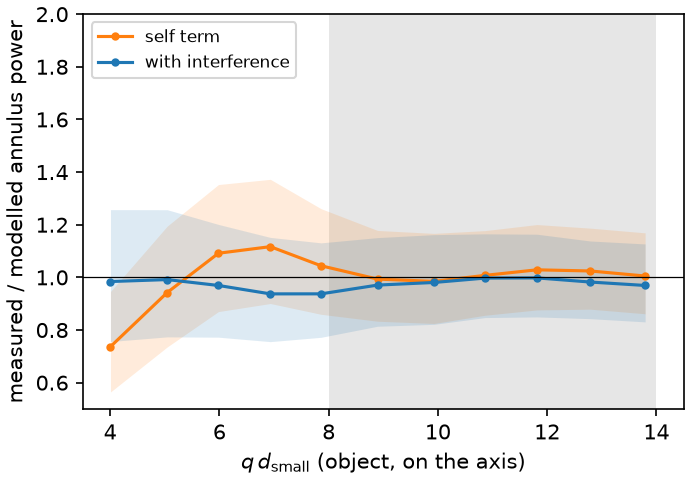
\includegraphics[width=0.6\linewidth]{spectra_check.png}
\caption{Measured patch spectra divided by the forward model evaluated on
the realised fields, for the self term only and with Percus--Yevick
interference at the mean composition. Lines are medians over all patches
and radiographs, bands the interquartile range. The shaded region is the
default band.}
\label{fig:spectra}
\end{figure}

Figure~\ref{fig:spectra} compares measured annulus values with
Eq.~\eqref{eq:additive} evaluated on the realised fields, so that it tests
the forward model alone. With the self term only, the median ratio runs from
$0.74$ at $q d_{\rm small}=4$ to $1.12$ near 7, where the first peak of the
structure factor of the small grains lies, and lies within $0.98$--$1.03$
above $q d_{\rm small}=9$. With interference included, the median ratio is
$0.94$--$1.00$ over the whole range. Within the default band the two models
differ by a few per cent, but in a pattern that varies across the band, and
including interference halves the species errors of the reconstruction
(Section~\ref{sec:default}).

\subsection{Default case}\label{sec:default}

\begin{figure}
\centering
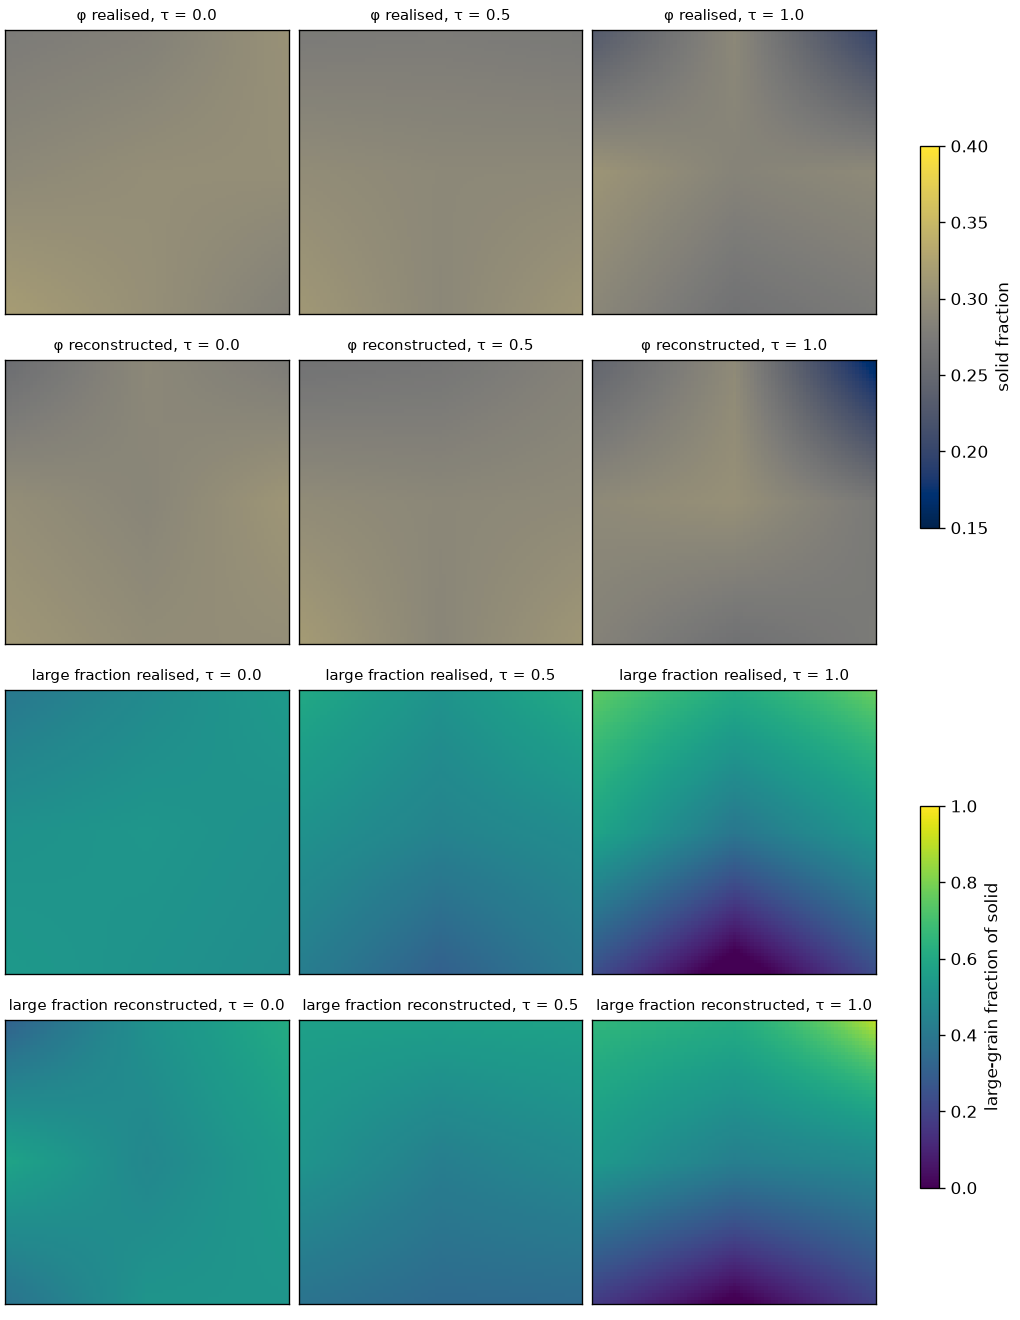
\includegraphics[width=0.75\linewidth]{segregation.png}
\caption{Vertical sections ($y=0$) through the realised and reconstructed
fields at the start, middle and end of the turn. Top two rows: solid
fraction. Bottom two rows: large-grain fraction of the solid.}
\label{fig:default}
\end{figure}

Figure~\ref{fig:default} shows vertical sections of the solid fraction and
the large-grain fraction at three times. The errors over the specimen and
the sequence are $0.0045$ in $\phi$, $0.0067$ and $0.0074$ in the small and
large volume fractions, $0.023$ in $c$ and $0.10$ voxels in $d_{32}$, which
ranges from 5 to 10 voxels. With the self term only they are $0.0125$,
$0.0126$, $0.042$ and $0.18$ voxels.

The errors of the two species are correlated, with coefficients between
$-0.6$ and $-0.8$ over the meshes tested. The patch means fix the total
$\phi$ closely, so an error in $\phi_{\rm large}$ reappears with the
opposite sign in $\phi_{\rm small}$. The independent outputs are therefore
$\phi$ and $c$.

\subsection{Grains per element}\label{sec:grains}

\begin{figure}
\centering
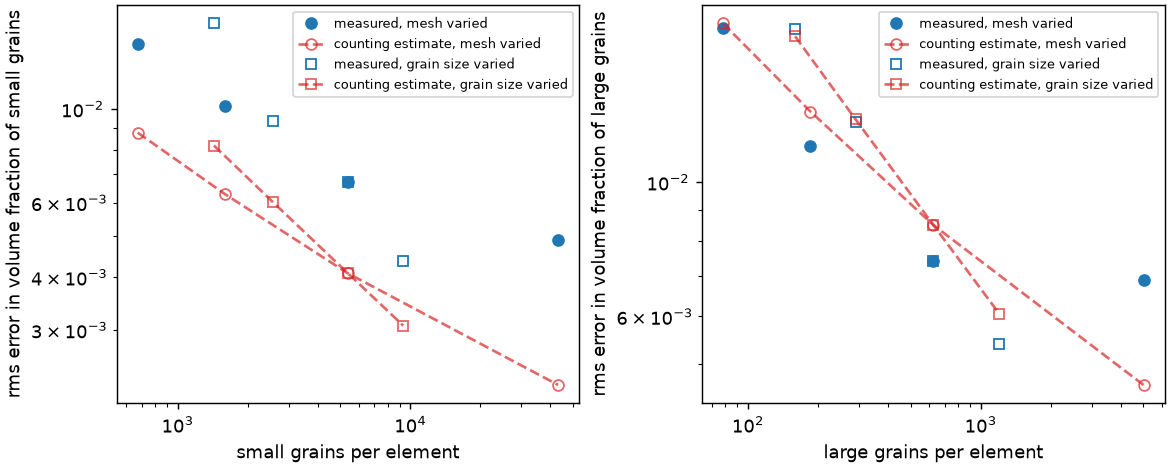
\includegraphics[width=0.9\linewidth]{grains_per_element.png}
\caption{Errors in the small (a) and large (b) volume fractions against the
number of grains of that species per element, with the mesh refined on the
same radiographs (filled) or the grains made smaller at a fixed mesh, with
pixel and patches scaled to keep the resolution per grain (open). Dashed
lines: counting estimate, Eq.~\eqref{eq:floor}.}
\label{fig:grains}
\end{figure}

The fields are defined at the scale of an element, and the number of
grains in an element fluctuates. For grains placed independently, the
least-squares fit of the grains onto the mesh has, at a point $\x$, variance
$\phi_a v_a\,\bm N(\x)^\top\mathsf M^{-1}\bm N(\x)$, where $\bm N$ are the
shape functions and $\mathsf M$ the mass matrix over the specimen
(Appendix~\ref{app:floor}). Hard spheres are placed more evenly than
independent points, and their count fluctuations are reduced by the partial
structure factor at zero wavenumber, so that
\begin{equation}
\operatorname{var}\phi_a(\x)=S_{aa}(0)\,\phi_a v_a\,\bm N(\x)^\top\mathsf M^{-1}\bm N(\x).
\label{eq:floor}
\end{equation}
Averaged over the specimen this is $\phi_a^2\,C\,S_{aa}(0)/n_a$, with $n_a$
the number of grains of species $a$ in an element and $C$ a constant of the
mesh and specimen shape, between $2.8$ and $5.1$ for the meshes with two or
more elements across the specimen and $11$ for a single element. For the default mixture
the Percus--Yevick values are $S_{\rm small}(0)=0.84$ and
$S_{\rm large}(0)=0.42$.

Figure~\ref{fig:grains} shows the errors of the two species against the
number of their grains per element, for meshes of 1 to 4 elements across
the specimen and for small grains of 4 to 8 voxels at a fixed mesh. The two
series fall on one curve. For the large grains the errors agree with
Eq.~\eqref{eq:floor}, which has no fitted parameter, from $0.018$ at 78
grains per element to $0.0054$ at 1200, and level off near $0.005$ for the
single-element mesh. The small-grain errors are $1.4$--$2.2$ times their own
estimate because they include the large-grain error through the total.
Equation~\eqref{eq:floor} therefore sets the element size for a required
accuracy, given the grain size and solid fraction.

\subsection{Detector, number of radiographs and size ratio}

\begin{table}
\centering
\caption{Error in the large-grain fraction of the solid, varying one setting
from the default.}
\label{tab:sensitivity}
\begin{tabular}{llc}
\toprule
Setting & Values & Error in $c$ \\
\midrule
Noise in $X$ (voxels) & 0, 0.3, 1, 3, 10 & 0.023, 0.023, 0.024, 0.025, 0.034 \\
Radiographs per turn & 90, 180, 360 & 0.023, 0.023, 0.023 \\
Pixel pitch (voxels) & 0.75, 1, 1.5 & 0.025, 0.023, 0.040 \\
Size ratio & 1.5, 2, 3 & 0.030, 0.023, 0.035 \\
Random seed & four seeds & 0.023--0.028 \\
\bottomrule
\end{tabular}
\end{table}

Table~\ref{tab:sensitivity} varies one setting at a time. Detector noise of
up to 3 voxels of path length per pixel, about 4\% of the path through the
centre, changes the error by less than $0.002$; at 10 voxels it rises to
$0.034$. Ninety, 180 and 360 radiographs per turn give the same errors, as
expected when the error is set by the grains per element. A pixel of
$1.5$ voxels limits the band to $q d_{\rm small}=6.9$--$8.9$, below the first
zero of the small grains' form factor and near the peak of their structure
factor, and the error rises to $0.040$; with the self term only it is
$0.164$. A larger size ratio separates the kernels of the two species more,
but at a fixed solid fraction it leaves fewer large grains per element (193
at a ratio of 3, 626 at 2), and the counting fluctuation increases the
error. The spread over four random seeds, $0.023$--$0.028$, sets the scale of
differences that can be resolved in these comparisons.

\subsection{Polydispersity}

When each species has a distribution of sizes, the kernel of a population
is the volume-weighted mean of Eq.~\eqref{eq:chia} over its sizes, with
interference among all of them. For two populations with Schulz size
distributions of coefficient of variation $0.25$ and $0.5$, each represented
by four sizes, the volume fraction errors are $0.009$--$0.016$ and $d_{32}$
is recovered to $0.18$--$0.25$ voxels, about twice the errors for single
sizes. A model with only the solid fraction and the specific surface, from
the Porod limit $\chi\to2\pi s/k^4$ \todo{cite: Porod law}, needs no
species. It gives $d_{32}$ to $0.20$ voxels for single sizes when the band
reaches $q d_{\rm small}=19$, but $0.62$--$0.64$ voxels for the size
distributions, whose smallest grains are not yet in the Porod regime at that
band.

\subsection{Time resolution}

\begin{table}
\centering
\caption{Error in $c$ for changes completed over a fraction $D$ of the turn,
against the number of time knots per turn, compared with a reference on a
fine time basis.}
\label{tab:time}
\begin{tabular}{lcccc}
\toprule
$D$ & 3 knots & 4 knots & 6 knots & 8 knots \\
\midrule
1 & 0.025 & 0.026 & 0.035 & 0.042 \\
0.5 & 0.033 & 0.025 & 0.037 & 0.042 \\
0.25 & 0.041 & 0.029 & 0.035 & 0.040 \\
\bottomrule
\end{tabular}
\end{table}

To test how fast the fields may change, the segregation and dilation were
compressed into a fraction $D$ of the turn, with 24 packings per turn.
Table~\ref{tab:time} gives the errors against the number of time knots. Four
knots follow a change over a quarter turn with an error of $0.029$, against
$0.026$ for a change spread over the whole turn. Three knots cannot follow
the quarter-turn change; six or eight knots add unknowns without adding
data and the errors grow. The errors at the first and last knots, which are
constrained by radiographs on one side only, are about twice those in the
middle of the sequence ($0.04$ against $0.02$), so the acquisition should
extend beyond the period of interest.

\subsection{Three dimensions against layers}\label{sec:layers}

\begin{figure}
\centering
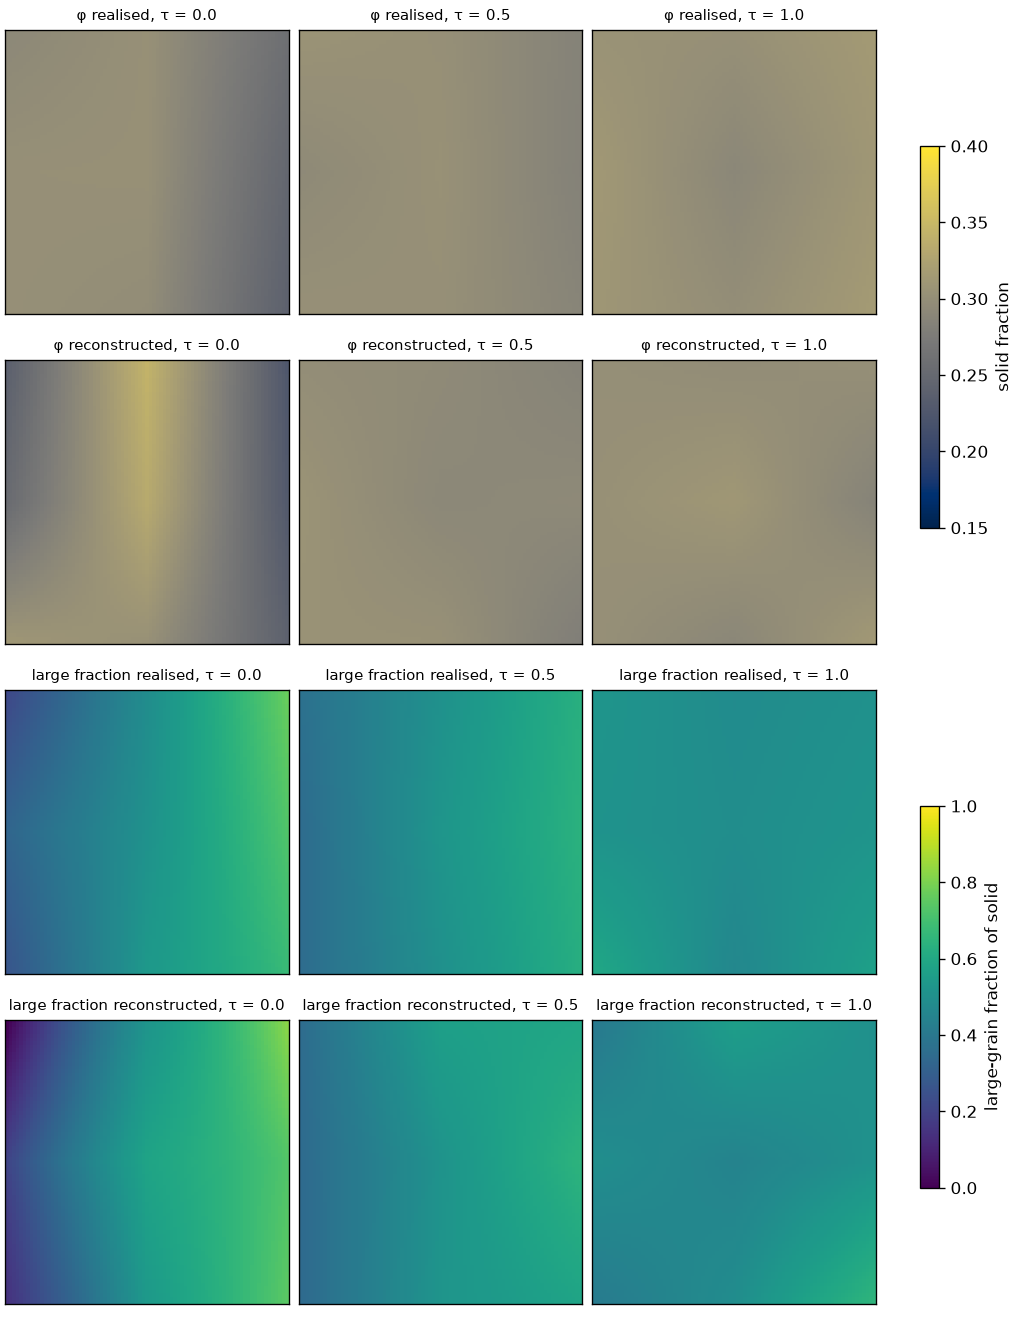
\includegraphics[width=0.75\linewidth]{rotating.png}
\caption{As Fig.~\ref{fig:default}, for side-to-side segregation whose
direction turns by $90^\circ$ during the sequence. The section is at $y=0$,
so the gradient lies in the section at the start and normal to it at the
end.}
\label{fig:rotating}
\end{figure}

\begin{table}
\centering
\caption{Error in $c$ for the 3D reconstruction and for fields constant
across each horizontal layer, fitted to the same radiographs and compared
with the same 3D reference.}
\label{tab:layers}
\begin{tabular}{lcc}
\toprule
Phantom & 3D & Layers only \\
\midrule
Segregation mainly with height (default) & 0.023 & 0.028--0.032 \\
Lateral segregation with a twist in height & 0.024 & 0.050 \\
Side-to-side segregation, direction turning by $90^\circ$ & 0.027 & 0.109 \\
\bottomrule
\end{tabular}
\end{table}

A method that assumes no variation across the beam could at best recover
fields that are constant across each horizontal layer. Table~\ref{tab:layers}
compares such fields, fitted to the same radiographs, with the 3D
reconstruction for three phantoms, and Fig.~\ref{fig:rotating} shows the
third. The benefit of the 3D reconstruction grows with the lateral
structure, to a factor of four. In the default phantom the lateral
structure of the realised fields, $0.008$ in $\phi_{\rm large}$, is no
larger than the reconstruction error, and the two approaches differ little.

\subsection{Local interference}\label{sec:local}

The kernels of Eq.~\eqref{eq:chia} were also evaluated at the local
large-grain fraction from the previous solution, interpolating between five
precomputed compositions. This changes the errors by less than $0.0002$ for
both the default and the lateral phantom, so the mean composition suffices
for large-grain fractions between $0.2$ and $0.8$.

\subsection{Container wall}\label{sec:wall}

Packings generated inside the container, without the larger cylinder,
carry the wall layer of sequential addition. Rays that graze the surface
cross it over long distances, and a smooth field cannot represent it. In the
interior, more than 20 voxels from the surface, the solid fraction error is
$0.011$ without a wall layer and $0.017$ with one. Adding, for each species,
a second field confined to a shell one large diameter thick at the wall
reduces it to $0.013$. Wall layers of real packings oscillate over a few
grain diameters \todo{cite: wall layering in packings}, and the shell model
has been tested only on synthetic packings.

\subsection{Uncertainty}

The posterior covariance of Eq.~\eqref{eq:ls}, scaled by the final
$\chi^2$, predicts errors three times smaller than observed, because the
realised fields themselves are defined only to the counting fluctuation of
Eq.~\eqref{eq:floor}. Adding that fluctuation to the posterior variance,
over four seeds, places 61--80\% of points within one predicted standard
deviation for $\phi$ and 64--74\% for $\phi_{\rm large}$, and 89--98\%
within two. For $\phi_{\rm small}$ the prediction must include the
large-grain fluctuation; taking the two as independent gives 85--89\%
within one standard deviation, a conservative bound.

% ---------------------------------------------------------------------------
\section{Experiments}\label{sec:experiments}

\plan{Static validation: a layered or graded bidisperse specimen scanned on
the DynaTOM and by full CT; ground truth $\phi_a(\x)$ from CT segmented by
grain size. Forward-model check on a homogeneous specimen at two or three
solid fractions. Dynamic case (percolation, silo discharge or tapping) with
full CT before and after. Detector processing: flat and dark correction,
linearisation including beam hardening, measured detector blur, calibrated
poses, container masking.}

% ---------------------------------------------------------------------------
\section{Discussion}

The method measures composition, not displacement. It needs no reference
scan and no persistence of the grain texture, so it applies to flows in
which grains rearrange. Its accuracy is set by the number of grains per
element, which is a property of the specimen and the chosen resolution, not
of the scanner, so that detector noise and the number of radiographs matter
little within the ranges tested. Equation~\eqref{eq:floor} gives the
trade-off between spatial resolution and accuracy before an experiment.

Three requirements follow from the tests. The detector must resolve the
small grains well enough that the band reaches $q d_{\rm small}\approx9$ or
higher, where the interference terms are small and well described by the
mean composition. The acquisition must extend beyond the period of
interest, because the first and last time knots are poorly constrained. The
container wall needs either a wall-layer term or exclusion of the surface
region from interpretation.

The tests have limits. The packings are built by sequential addition, not
by flow, and their structure factors are close to, but not the same as,
those of the Percus--Yevick closure. Real data add beam hardening, scatter,
detector blur and the container, none of which are modelled here. The
time resolution is tested for changes that are smooth in space.

Species velocities are not measured. Consecutive radiographs differ in
angle, so the cross-spectrum between them mixes the motion of the grains
with a parallax that varies with depth; at the angular steps of a typical
rotation this parallax exceeds a small grain's diameter. The reconstructed
fields do, however, constrain the fluxes through the conservation of each
species, $\partial_\tau\phi_a+\nabla\cdot(\phi_a\bm u_a)=0$, which is a
natural extension.

% ---------------------------------------------------------------------------
\section{Conclusions}

The spectrum of a radiograph patch of a dense granular mixture is, in
expectation, a line integral of a local spectral density linear in the
species volume fractions, with grain interference included through
partial structure factors at the mean composition. Radiographs from a
rotating scanner then determine three-dimensional, time-dependent fields of
solid fraction and composition by linear least squares. On synthetic
radiographs of evolving bidisperse packings, the solid fraction is
recovered to $0.005$ and the large-grain fraction to $0.023$ with about 600
large grains per element, the large-grain error equals the counting
fluctuation of the grains without a fitted parameter, and the 3D
reconstruction reduces the error of layer-wise fields by up to a factor of
four. The method is limited by the number of grains per element, by a
detector band reaching $q d_{\rm small}\approx9$ and by the ends of the
acquisition. \todo{experimental conclusions} The next step is to use the
fields to constrain species fluxes through mass conservation.

% ---------------------------------------------------------------------------
\appendix
\section{Counting fluctuation of a projected field}\label{app:floor}

Let the realised field of species $a$ be the least-squares fit
$\tilde\phi_a(\x)=\bm N(\x)^\top\mathsf M^{-1}\bm b$, with
$\mathsf M=\int\bm N\bm N^\top\dd V$ over the specimen and
$\bm b=\sum_j v_a\bm N(\x_j)$ over the grains $j$ of species $a$. For grain
centres forming a stationary point process of density $\rho_a$ with
structure factor $S_{aa}$, and shape functions varying slowly on the scale
of the grain spacing,
$\operatorname{cov}\bm b=\rho_a v_a^2 S_{aa}(0)\,\mathsf M$. Hence
$\operatorname{var}\tilde\phi_a(\x)=\rho_a v_a^2 S_{aa}(0)\,\bm N^\top\mathsf
M^{-1}\bm N=S_{aa}(0)\,\phi_a v_a\,\bm N^\top\mathsf M^{-1}\bm N$, which is
Eq.~\eqref{eq:floor}.

\section*{Code and data availability}
The method and the synthetic tests are implemented in \texttt{pynamix}
(modules \texttt{pynamix.spectral.tomography} and \texttt{pynamix.pdvc},
scripts in \texttt{examples/pdvc}) \todo{repository link and version}.

\end{document}
